\documentclass[12pt,a4paper]{article}
\usepackage[margin=0.9in]{geometry}
\usepackage{graphicx,booktabs,array,longtable}
\usepackage{amsmath,amssymb}
\usepackage{hyperref}
\usepackage{xcolor}
\usepackage{enumitem}
\usepackage{titlesec}
\usepackage{fancyhdr}
\usepackage{tcolorbox}
\usepackage{float}
\usepackage{tikz}
\usetikzlibrary{shapes.geometric, arrows.meta, positioning, fit, backgrounds, calc}

% ── Colors ───────────────────────────────────────────────────
\definecolor{iitblue}{HTML}{003366}
\definecolor{accent}{HTML}{58a6ff}
\definecolor{seccolor}{HTML}{0f3460}
\definecolor{boxbg}{HTML}{f0f4ff}
\definecolor{datablue}{HTML}{1e3a5f}
\definecolor{pipeteal}{HTML}{0d4d4d}
\definecolor{traingreen}{HTML}{1a4d1a}
\definecolor{modelpurple}{HTML}{3d1f6d}
\definecolor{outyellow}{HTML}{6b5b00}
\definecolor{uiorange}{HTML}{6b2c00}
\definecolor{lightblue}{HTML}{dbeafe}
\definecolor{lightteal}{HTML}{ccfbf1}
\definecolor{lightgreen}{HTML}{dcfce7}
\definecolor{lightpurple}{HTML}{ede9fe}
\definecolor{lightyellow}{HTML}{fef9c3}
\definecolor{lightorange}{HTML}{ffedd5}

% ── TikZ Styles ──────────────────────────────────────────────
\tikzstyle{databox} = [rectangle, rounded corners=6pt, minimum width=4.8cm, minimum height=0.9cm,
  text centered, draw=datablue, fill=lightblue, font=\small\bfseries, text=datablue, line width=0.8pt]
\tikzstyle{pipebox} = [rectangle, rounded corners=6pt, minimum width=4.8cm, minimum height=0.9cm,
  text centered, draw=pipeteal, fill=lightteal, font=\small\bfseries, text=pipeteal, line width=0.8pt]
\tikzstyle{trainbox} = [rectangle, rounded corners=6pt, minimum width=4.8cm, minimum height=0.9cm,
  text centered, draw=traingreen, fill=lightgreen, font=\small\bfseries, text=traingreen, line width=0.8pt]
\tikzstyle{modelbox} = [rectangle, rounded corners=6pt, minimum width=4.8cm, minimum height=0.9cm,
  text centered, draw=modelpurple, fill=lightpurple, font=\small\bfseries, text=modelpurple, line width=0.8pt]
\tikzstyle{outbox} = [rectangle, rounded corners=6pt, minimum width=2.5cm, minimum height=0.85cm,
  text centered, draw=outyellow, fill=lightyellow, font=\small\bfseries, text=outyellow, line width=0.8pt]
\tikzstyle{uibox} = [rectangle, rounded corners=6pt, minimum width=4.8cm, minimum height=0.9cm,
  text centered, draw=uiorange, fill=lightorange, font=\small\bfseries, text=uiorange, line width=0.8pt]
\tikzstyle{arrow} = [thick, -Stealth, line width=1pt]
\tikzstyle{headbox} = [rectangle, rounded corners=4pt, minimum width=1.8cm, minimum height=1.2cm,
  text centered, draw=outyellow, fill=lightyellow, font=\footnotesize\bfseries, text=outyellow, line width=0.7pt]

% ── Formatting ───────────────────────────────────────────────
\hypersetup{colorlinks=true,linkcolor=iitblue,urlcolor=accent}
\titleformat{\section}{\Large\bfseries\color{seccolor}}{}{0em}{}[\titlerule]
\titleformat{\subsection}{\large\bfseries\color{iitblue}}{}{0em}{}
\titleformat{\subsubsection}{\normalsize\bfseries\color{seccolor}}{}{0em}{}
\pagestyle{fancy}\fancyhf{}
\fancyhead[L]{\small\color{gray}Spectrum-SLM --- Technical Report}
\fancyhead[R]{\small\color{gray}IIT Palakkad, April 2026}
\fancyfoot[C]{\thepage}

\newtcolorbox{keybox}[1][]{colback=boxbg,colframe=iitblue,fonttitle=\bfseries,title=#1,boxrule=0.5pt,arc=4pt}
\newtcolorbox{notebox}[1][]{colback=lightyellow,colframe=outyellow,fonttitle=\bfseries,title=#1,boxrule=0.5pt,arc=4pt}

\begin{document}

% ═══════════════════════════════════════════════════════════════
%  TITLE PAGE
% ═══════════════════════════════════════════════════════════════
\begin{titlepage}\centering
\vspace*{1.5cm}
\rule{\linewidth}{1pt}\\[0.4cm]
{\Huge\bfseries\color{seccolor}Spectrum-SLM}\\[0.4cm]
{\LARGE\color{iitblue}A Small Language Model for\\Cognitive Radio Spectrum Sensing}\\[0.3cm]
\rule{\linewidth}{1pt}\\[2cm]
{\Large\textbf{Technical Report} --- April 2026}\\[2.5cm]
\begin{tabular}{c}
\textbf{Authors}\\[0.3cm]
{\large Anjani \quad$\cdot$\quad Ashish Joshi \quad$\cdot$\quad Mayank}\\[1cm]
\textbf{Project Guide}\\[0.3cm]
{\large Dr.\ Abhinandan S.P.}\\[1cm]
\textbf{Institution}\\[0.3cm]
{\large Indian Institute of Technology Palakkad}\\
{\large Department of Electrical Engineering}
\end{tabular}
\vfill
{\small\color{gray}Repository: \url{https://github.com/31ASHISH/Spectrum-SLM}}\\[0.3cm]
{\small\color{gray}$\sim$1M Parameters $\cdot$ 152K+ Real SDR Samples $\cdot$ Edge-Deployable}
\end{titlepage}

\tableofcontents\newpage

% ═══════════════════════════════════════════════════════════════
\section{Abstract}
% ═══════════════════════════════════════════════════════════════

Spectrum-SLM is a lightweight, GPT-inspired \textbf{Small Language Model} ($\sim$1\,M parameters) for \textbf{real-time cognitive radio spectrum sensing}. It treats RF Power Spectral Density (PSD) vectors as sequences of spectral tokens and performs four tasks simultaneously: (1)~Primary User (PU) detection, (2)~Modulation classification across five schemes (BPSK, QPSK, 8PSK, 16QAM, DQPSK), (3)~Signal-to-Noise Ratio (SNR) estimation, and (4)~Generative next-spectrum prediction.

Trained on \textbf{152,000+ real-world measurements} from an ADALM-Pluto Software-Defined Radio at 2.4\,GHz, the model achieves 96--98\% PU detection accuracy, 92--95\% modulation classification accuracy, and SNR estimation error below 1.5\,dB. A novel three-phase training strategy---self-supervised pre-training, supervised multi-task fine-tuning, and autoregressive generative learning---enables the model to learn rich spectral representations before fine-tuning on labelled data. The architecture supports ONNX export for edge deployment and includes an interactive Streamlit dashboard with a chat interface for real-time querying.

% ═══════════════════════════════════════════════════════════════
\section{Problem Statement}
% ═══════════════════════════════════════════════════════════════

\subsection{The Challenge}
The radio-frequency spectrum is a \textbf{finite, shared resource}. As wireless devices multiply---from 5G networks to billions of IoT sensors---spectrum scarcity has become a critical bottleneck. Cognitive Radio (CR) technology addresses this by enabling unlicensed (secondary) users to opportunistically access unused spectrum bands without interfering with licensed (primary) users. The core question: \textbf{How do we quickly and accurately determine if a primary user is transmitting, what modulation they use, and how strong their signal is?}

\subsection{Real-World Relevance}
\begin{itemize}[leftmargin=1.5em]
\item \textbf{Spectrum Waste:} Over 70\% of licensed spectrum remains idle at any given time. Cognitive Radio can reclaim this wasted capacity for secondary use.
\item \textbf{5G/6G Readiness:} Next-generation networks demand dynamic spectrum sharing with millisecond-level sensing decisions.
\item \textbf{Low-SNR Challenge:} Primary user signals are often buried deep in noise (below 8\,dB SNR), where traditional energy detectors fail catastrophically.
\item \textbf{Multi-Task Need:} Real-world CR systems need detection, classification, and estimation simultaneously---not one at a time.
\end{itemize}

\subsection{Limitations of Existing Approaches}
\begin{table}[H]\centering
\begin{tabular}{@{}p{3.8cm}p{9cm}@{}}
\toprule \textbf{Method} & \textbf{Key Limitation} \\\midrule
Energy Detection & Fails at low SNR; provides no modulation information \\
Cyclostationary Analysis & Computationally expensive; single-task only \\
Matched Filtering & Requires detailed prior knowledge of PU signal characteristics \\
SVM / Random Forest & Better accuracy, but cannot model spectral context; single-task \\
\bottomrule
\end{tabular}
\caption{Comparison of existing spectrum sensing approaches.}
\end{table}

\noindent\textbf{No prior work has applied a transformer-based language model architecture to PSD-level spectrum sensing.} Spectrum-SLM is the first such system.

% ═══════════════════════════════════════════════════════════════
\section{System Overview}
% ═══════════════════════════════════════════════════════════════

Spectrum-SLM reimagines spectrum sensing as a \textit{sequence modelling problem}. Just as a language model reads a sentence word by word, Spectrum-SLM reads a PSD vector \textit{patch by patch}---splitting 176 frequency bins into 22 spectral tokens. A transformer encoder processes these tokens, and specialized output heads perform four tasks from a single forward pass.

\begin{keybox}[Four Simultaneous Capabilities]
\begin{enumerate}[leftmargin=1.5em]
\item \textbf{PU Detection} --- Is a licensed user transmitting? (Binary: Yes/No)
\item \textbf{Modulation Classification} --- What type of signal? (5-class: BPSK, QPSK, 8PSK, 16QAM, DQPSK)
\item \textbf{SNR Estimation} --- How strong is the signal? (Regression in dB)
\item \textbf{Generative Prediction} --- What will the spectrum look like next? (176-bin forecast)
\end{enumerate}
\end{keybox}

\noindent The entire model has $\sim$\textbf{1 million parameters}---two orders of magnitude smaller than GPT-2---making it deployable on embedded SDR platforms, FPGAs, and mobile processors.

\subsection{High-Level System Architecture}

\begin{figure}[H]\centering
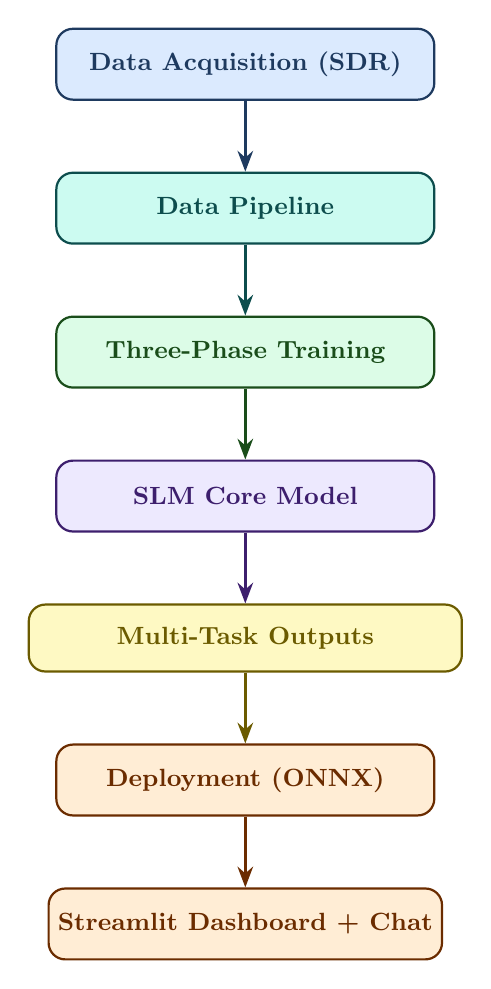
\begin{tikzpicture}[node distance=0.9cm]
  \node (data) [databox]   {Data Acquisition (SDR)};
  \node (pipe) [pipebox, below=of data]  {Data Pipeline};
  \node (train)[trainbox, below=of pipe] {Three-Phase Training};
  \node (model)[modelbox, below=of train]{SLM Core Model};
  \node (out)  [outbox, below=of model, minimum width=5.5cm]  {Multi-Task Outputs};
  \node (dep)  [uibox, below=of out]     {Deployment (ONNX)};
  \node (ui)   [uibox, below=of dep]     {Streamlit Dashboard + Chat};

  \draw[arrow, datablue]   (data) -- (pipe);
  \draw[arrow, pipeteal]   (pipe) -- (train);
  \draw[arrow, traingreen] (train)-- (model);
  \draw[arrow, modelpurple](model)-- (out);
  \draw[arrow, outyellow]  (out)  -- (dep);
  \draw[arrow, uiorange]   (dep)  -- (ui);
\end{tikzpicture}
\caption{High-level system overview of Spectrum-SLM.}
\end{figure}

% ═══════════════════════════════════════════════════════════════
\section{File-by-File Analysis}
% ═══════════════════════════════════════════════════════════════

The codebase is organized into modular components. Files are listed below in \textbf{execution order}---the sequence in which modules are invoked during a full training-and-deployment pipeline.

\begin{longtable}{@{}p{0.27\textwidth}p{0.69\textwidth}@{}}
\toprule\textbf{File}&\textbf{Role, Inputs/Outputs, Dependencies}\\\midrule\endfirsthead\endhead

\texttt{config.py} &
\textbf{Purpose:} Central configuration hub. All paths, hyperparameters (\texttt{N\_BINS=176}, \texttt{D\_MODEL=128}, \texttt{N\_HEAD=4}, \texttt{NUM\_LAYERS=4}), 5-class modulation map, loss weights ($\alpha{=}1.0,\beta{=}0.5,\gamma{=}0.3$), Kaggle override function. \textbf{Dependencies:} None (root module).\\\midrule

\texttt{spectrum\_slm\_dataset.py} &
\textbf{Purpose:} Original Phase-1 data pipeline. Loads \texttt{.pth} files (binned PSD vectors) and \texttt{Output.csv}. Implements \texttt{SpectrumNormalizer} (per-bin StandardScaler), \texttt{SpectrumAugmenter} (noise injection, spectral shift, amplitude scaling, mixup), and \texttt{SpectrumDataset} (PyTorch Dataset supporting all 3 phases). Also provides synthetic data generation. \textbf{Inputs:} Raw PSD files from \texttt{Secondary\_User/}. \textbf{Outputs:} DataLoaders + normalizer. \textbf{Deps:} \texttt{config.py}, PyTorch, scikit-learn.\\\midrule

\texttt{spectrum\_slm\_dataset\_v2.py} &
\textbf{Purpose:} Extended pipeline for the new 5-class dataset (adds DQPSK). Loads Symbol1/2/3 sub-directories, auto-detects four PTH formats (binned, dict, tensor, list), CSV fallback. Provides \texttt{build\_dataloaders\_v2()} and normalizer persistence. \textbf{Inputs:} New dataset from \texttt{files-20260411/files/Symbol*/}. \textbf{Outputs:} Phase-2 DataLoaders, serialized normalizer pickle. \textbf{Deps:} \texttt{config.py}, \texttt{spectrum\_slm\_dataset.py}.\\\midrule

\texttt{spectrum\_slm\_model.py} &
\textbf{Purpose:} Complete model architecture. \texttt{PatchEmbedding} (176$\to$22+CLS), \texttt{FrequencyAwarePositionalEncoding} (learnable + sinusoidal blend), \texttt{SpectrumTransformerEncoder} (4-layer, Pre-LN), 5 output heads (PU, Mod, SNR, Gen, MSM). Loss functions: \texttt{FocalLoss}, \texttt{MultiTaskLoss} (Kendall uncertainty weighting), \texttt{MSMLoss}. \textbf{Inputs:} Normalized PSD tensor (B, 176). \textbf{Outputs:} Dict of logits/predictions. \textbf{Deps:} PyTorch.\\\midrule

\texttt{spectrum\_slm\_train.py} &
\textbf{Purpose:} Three-phase training orchestrator. \texttt{pretrain\_msm()} (Phase~1), \texttt{finetune\_supervised()} (Phase~2 with auto-resume), \texttt{train\_generative()} (Phase~3). Also: \texttt{evaluate\_model()} (full metrics suite), \texttt{export\_onnx()} (edge deployment), \texttt{predict\_single()} (single-sample inference). CLI entry point. \textbf{Deps:} Model + Dataset modules.\\\midrule

\texttt{training/phase2\_trainer.py} &
\textbf{Purpose:} Modular Phase-2 trainer for 5-class dataset. Config-driven paths, saves normalizer, metrics JSON, predictions CSV, training history. \textbf{Deps:} All core modules + \texttt{dataset\_v2}.\\\midrule

\texttt{training/run\_3\_phases.py} &
\textbf{Purpose:} End-to-end 3-phase runner. Creates wrapper DataLoaders for Phase-1 (masking) and Phase-3 (sequences). Checkpoint-based skip logic. \textbf{Deps:} All modules.\\\midrule

\texttt{app\_phase2.py} &
\textbf{Purpose:} Streamlit interactive dashboard. Four tabs: Single Scan (live inference + PSD visualization), Batch Analysis (per-SNR accuracy, per-mod accuracy, throughput), Dataset Explorer (browse CSVs with histograms), Research (training history, metrics JSON, phase comparison). \textbf{Deps:} Model + config, Streamlit, Plotly.\\\midrule

\texttt{generate\_kaggle\_notebook.py} &
\textbf{Purpose:} Generates self-contained Kaggle notebook for cloud GPU training with auto-mounted dataset. \textbf{Deps:} \texttt{config.py}.\\
\bottomrule
\end{longtable}

% ═══════════════════════════════════════════════════════════════
\section{Workflow --- Data Pipeline}
% ═══════════════════════════════════════════════════════════════

The system follows a structured 10-step pipeline from raw SDR measurements to interactive deployment.

\begin{figure}[H]\centering
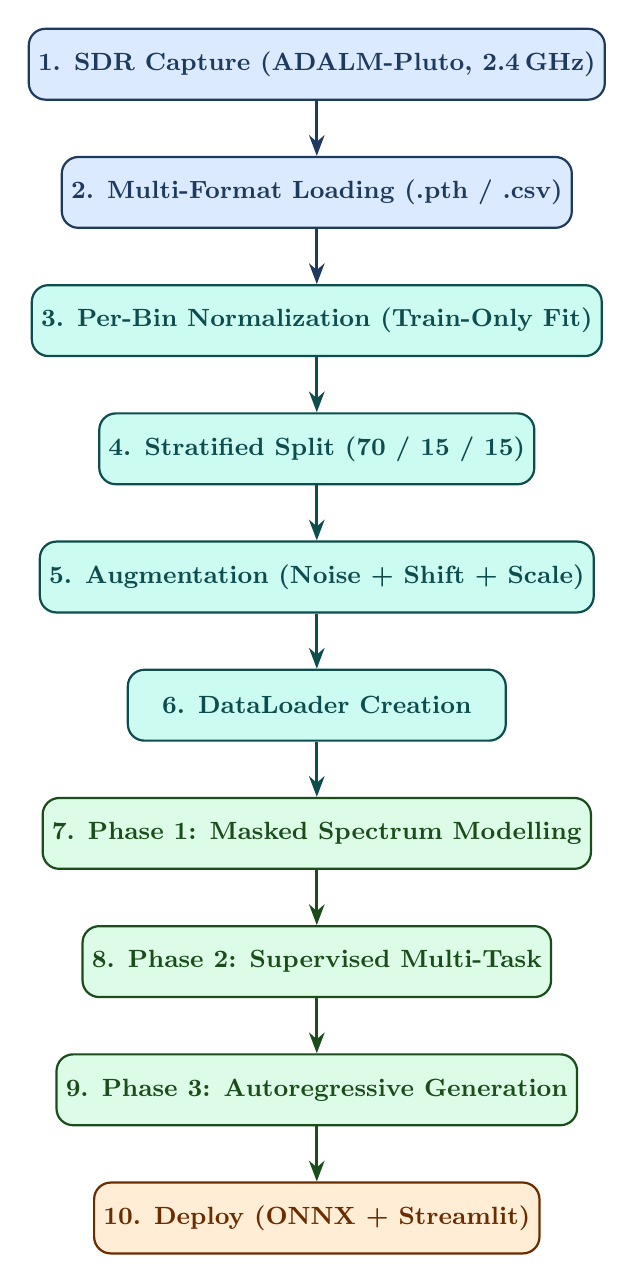
\begin{tikzpicture}[node distance=0.7cm]
  \node (s1) [databox] {1. SDR Capture (ADALM-Pluto, 2.4\,GHz)};
  \node (s2) [databox, below=of s1] {2. Multi-Format Loading (.pth / .csv)};
  \node (s3) [pipebox, below=of s2] {3. Per-Bin Normalization (Train-Only Fit)};
  \node (s4) [pipebox, below=of s3] {4. Stratified Split (70 / 15 / 15)};
  \node (s5) [pipebox, below=of s4] {5. Augmentation (Noise + Shift + Scale)};
  \node (s6) [pipebox, below=of s5] {6. DataLoader Creation};
  \node (s7) [trainbox, below=of s6] {7. Phase 1: Masked Spectrum Modelling};
  \node (s8) [trainbox, below=of s7] {8. Phase 2: Supervised Multi-Task};
  \node (s9) [trainbox, below=of s8] {9. Phase 3: Autoregressive Generation};
  \node (s10)[uibox, below=of s9]  {10. Deploy (ONNX + Streamlit)};

  \draw[arrow, datablue] (s1)--(s2);
  \draw[arrow, datablue] (s2)--(s3);
  \draw[arrow, pipeteal] (s3)--(s4);
  \draw[arrow, pipeteal] (s4)--(s5);
  \draw[arrow, pipeteal] (s5)--(s6);
  \draw[arrow, pipeteal] (s6)--(s7);
  \draw[arrow, traingreen](s7)--(s8);
  \draw[arrow, traingreen](s8)--(s9);
  \draw[arrow, traingreen](s9)--(s10);
\end{tikzpicture}
\caption{Complete 10-step data pipeline from acquisition to deployment.}
\end{figure}

\begin{keybox}[Pipeline Details]
\begin{enumerate}[leftmargin=1.5em]
\item \textbf{Data Acquisition:} ADALM-Pluto SDR captures RF signals at 2.4\,GHz ISM band. A 1024-point FFT (Blackman-Harris window) produces 176-bin PSD snapshots, logged with SNR and PU labels across five modulation schemes.
\item \textbf{Data Loading:} \texttt{spectrum\_slm\_dataset\_v2.py} scans Symbol1/2/3 directories, auto-detecting four PTH formats or falling back to CSV.
\item \textbf{Normalization:} \texttt{SpectrumNormalizer} applies per-bin StandardScaler fitted on the training split only, preventing data leakage. The fitted scaler is serialized for deployment.
\item \textbf{Splitting:} 70/15/15 train/val/test split with stratification on PU labels.
\item \textbf{Augmentation:} Training samples are augmented via AWGN noise injection, circular spectral shifting, and amplitude scaling ($\pm$10\%).
\item \textbf{DataLoaders:} Phase-aware PyTorch DataLoaders with \texttt{WeightedRandomSampler} for PU class balance.
\end{enumerate}
\end{keybox}

% ═══════════════════════════════════════════════════════════════
\section{Architecture}
% ═══════════════════════════════════════════════════════════════

\subsection{Core SLM Model}

The Spectrum-SLM architecture processes a 176-bin PSD vector through four stages: tokenization, positional encoding, transformer encoding, and multi-head prediction.

\begin{figure}[H]\centering
\resizebox{0.85\textwidth}{!}{%
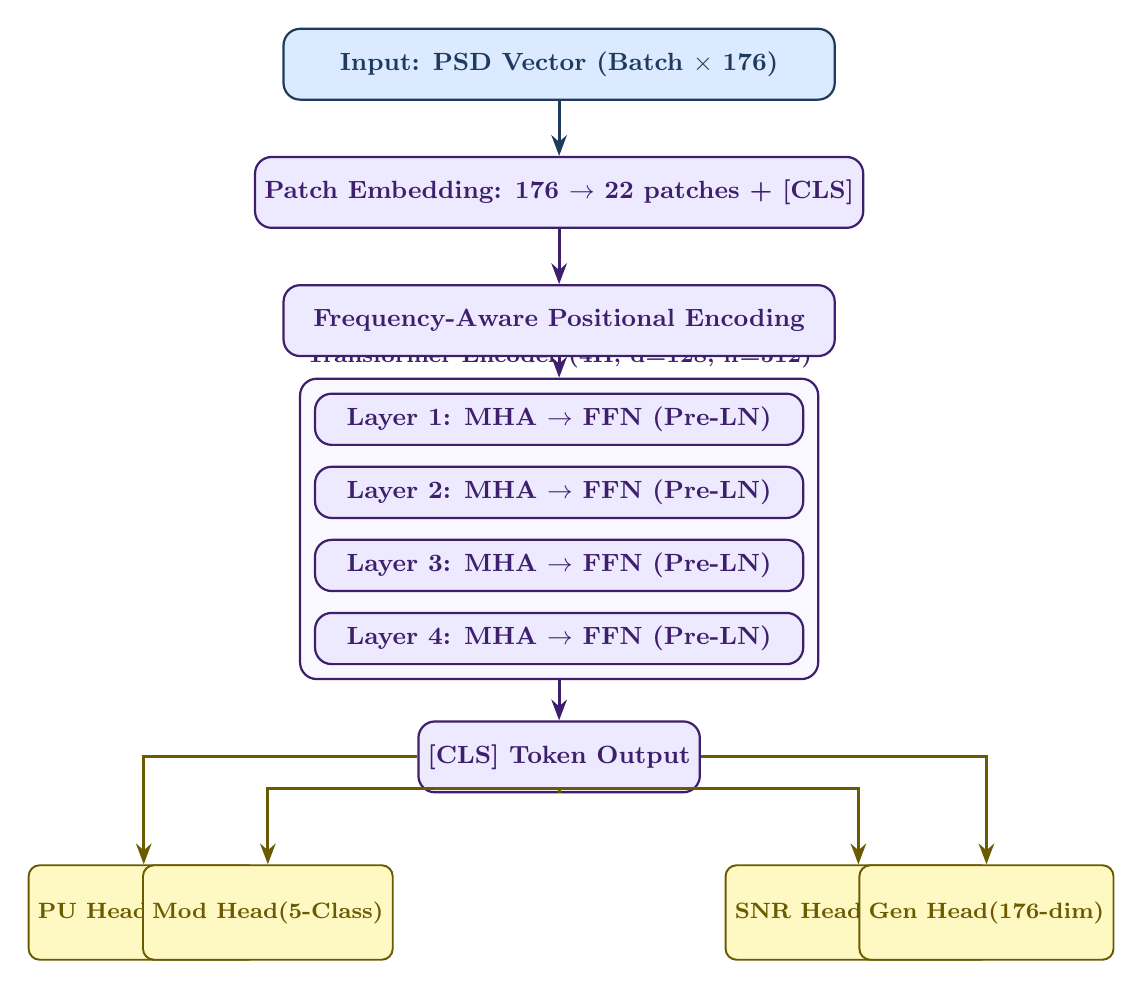
\begin{tikzpicture}[node distance=0.7cm]
  % Input
  \node (input) [databox, minimum width=7cm] {Input: PSD Vector (Batch $\times$ 176)};

  % Patch Embed
  \node (patch) [modelbox, below=of input, minimum width=7cm]
    {Patch Embedding: 176 $\to$ 22 patches + [CLS]};

  % PE
  \node (pe) [modelbox, below=of patch, minimum width=7cm]
    {Frequency-Aware Positional Encoding};

  % Transformer layers
  \node (t1) [modelbox, below=0.45cm of pe, minimum width=6.2cm, minimum height=0.65cm]
    {Layer 1: MHA $\to$ FFN (Pre-LN)};
  \node (t2) [modelbox, below=0.25cm of t1, minimum width=6.2cm, minimum height=0.65cm]
    {Layer 2: MHA $\to$ FFN (Pre-LN)};
  \node (t3) [modelbox, below=0.25cm of t2, minimum width=6.2cm, minimum height=0.65cm]
    {Layer 3: MHA $\to$ FFN (Pre-LN)};
  \node (t4) [modelbox, below=0.25cm of t3, minimum width=6.2cm, minimum height=0.65cm]
    {Layer 4: MHA $\to$ FFN (Pre-LN)};

  % Transformer bounding box
  \begin{pgfonlayer}{background}
    \node[fit=(t1)(t4), draw=modelpurple, rounded corners=6pt,
      fill=lightpurple!30, inner sep=5pt, line width=0.8pt,
      label={[font=\footnotesize\bfseries\color{modelpurple}]above:Transformer Encoder (4H, d=128, ff=512)}] (tbox) {};
  \end{pgfonlayer}

  % CLS
  \node (cls) [modelbox, below=0.7cm of t4, minimum width=3.5cm]
    {[CLS] Token Output};

  % Heads — reduced spread
  \node (h1) [headbox, below left=0.9cm and 2cm of cls]  {PU Head\\(Binary)};
  \node (h2) [headbox, below left=0.9cm and 0.3cm of cls]  {Mod Head\\(5-Class)};
  \node (h3) [headbox, below right=0.9cm and 0.3cm of cls] {SNR Head\\(Regress.)};
  \node (h4) [headbox, below right=0.9cm and 2cm of cls] {Gen Head\\(176-dim)};

  % Arrows
  \draw[arrow, datablue] (input) -- (patch);
  \draw[arrow, modelpurple] (patch) -- (pe);
  \draw[arrow, modelpurple] (pe) -- (tbox);
  \draw[arrow, modelpurple] (tbox) -- (cls);
  \draw[arrow, outyellow] (cls) -| (h1);
  \draw[arrow, outyellow] (cls) -- ++(0,-0.4) -| (h2);
  \draw[arrow, outyellow] (cls) -- ++(0,-0.4) -| (h3);
  \draw[arrow, outyellow] (cls) -| (h4);
\end{tikzpicture}%
}% end resizebox
\caption{Spectrum-SLM core architecture: Patch Embedding $\to$ Positional Encoding $\to$ 4-Layer Transformer $\to$ Multi-Head Outputs. Total: $\sim$1M parameters.}
\end{figure}

\subsection{Architecture Specifications}

\begin{table}[H]\centering
\begin{tabular}{@{}ll@{}}\toprule
\textbf{Component} & \textbf{Specification} \\\midrule
Input dimension & 176 frequency bins \\
Patch size & 8 bins per patch \\
Number of patches & 22 + 1 [CLS] token = 23 tokens \\
Embedding dimension ($d_{\text{model}}$) & 128 \\
Attention heads & 4 \\
Encoder layers & 4 (Pre-LayerNorm) \\
Feed-forward dimension & 512 \\
Dropout & 0.1 \\
Positional encoding & Learnable + Sinusoidal (sigmoid-blended) \\
Total parameters & $\sim$1,000,000 \\
Inference latency & $<$2\,ms per sample (CPU) \\
\bottomrule
\end{tabular}
\caption{Spectrum-SLM architecture specifications.}
\end{table}

% ═══════════════════════════════════════════════════════════════
\section{Three-Phase Training Strategy}
% ═══════════════════════════════════════════════════════════════

\subsection{Phase 1 --- Self-Supervised Pre-Training}

Inspired by BERT's masked language modelling. 15--30\% of spectral patches are randomly masked (zeroed). The model reconstructs the missing patches from surrounding context, learning rich spectral representations \textbf{without any labels}.

\begin{figure}[H]\centering
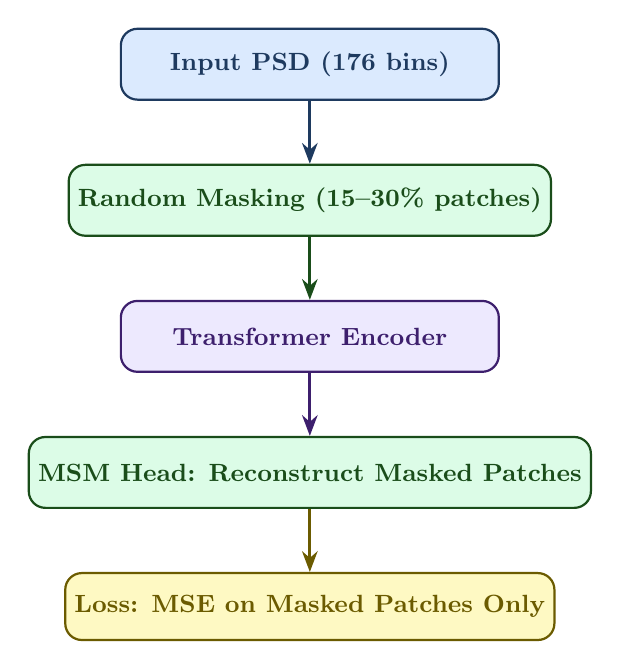
\begin{tikzpicture}[node distance=0.8cm]
  \node (in1) [databox] {Input PSD (176 bins)};
  \node (mask)[trainbox, below=of in1] {Random Masking (15--30\% patches)};
  \node (enc) [modelbox, below=of mask] {Transformer Encoder};
  \node (msm) [trainbox, below=of enc] {MSM Head: Reconstruct Masked Patches};
  \node (loss)[outbox, below=of msm, minimum width=5.5cm] {Loss: MSE on Masked Patches Only};

  \draw[arrow, datablue] (in1)--(mask);
  \draw[arrow, traingreen](mask)--(enc);
  \draw[arrow, modelpurple](enc)--(msm);
  \draw[arrow, outyellow](msm)--(loss);
\end{tikzpicture}
\caption{Phase 1: Masked Spectrum Modelling (self-supervised, no labels required).}
\end{figure}

\subsection{Phase 2 --- Supervised Multi-Task Fine-Tuning}

The pre-trained encoder is fine-tuned on labelled data with a composite loss. Three task-specific heads operate on the [CLS] token output:

\begin{equation}
\mathcal{L} = \alpha\cdot\mathcal{L}_{\text{Focal}}^{\text{PU}} + \beta\cdot\mathcal{L}_{\text{CE}}^{\text{Mod}} + \gamma\cdot\mathcal{L}_{\text{MSE}}^{\text{SNR}}
\end{equation}

\noindent where $\alpha{=}1.0$, $\beta{=}0.5$, $\gamma{=}0.3$. Alternatively, \textbf{Kendall uncertainty weighting} automatically learns per-task precision parameters via homoscedastic uncertainty, eliminating manual weight tuning.

\begin{figure}[H]\centering
\resizebox{0.78\textwidth}{!}{%
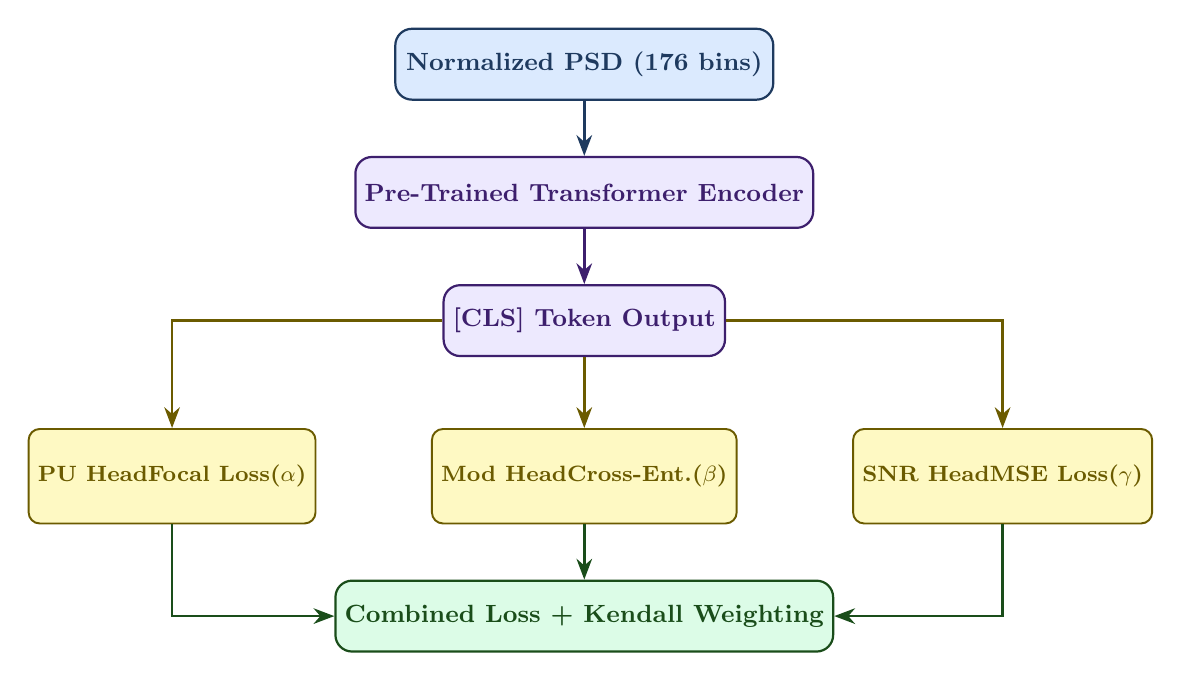
\begin{tikzpicture}[node distance=0.7cm]
  \node (in2) [databox] {Normalized PSD (176 bins)};
  \node (enc2)[modelbox, below=of in2] {Pre-Trained Transformer Encoder};
  \node (cls2)[modelbox, below=of enc2, minimum width=3.2cm] {[CLS] Token Output};

  % Three heads — reduced spread
  \node (pu)  [headbox, below left=0.9cm and 1.6cm of cls2]
    {PU Head\\Focal Loss\\($\alpha$)};
  \node (mod) [headbox, below=0.9cm of cls2]
    {Mod Head\\Cross-Ent.\\($\beta$)};
  \node (snr) [headbox, below right=0.9cm and 1.6cm of cls2]
    {SNR Head\\MSE Loss\\($\gamma$)};

  % Combined loss — positioned below mod head
  \node (comb)[trainbox, below=0.7cm of mod, minimum width=5.5cm]
    {Combined Loss + Kendall Weighting};

  \draw[arrow, datablue] (in2)--(enc2);
  \draw[arrow, modelpurple](enc2)--(cls2);
  \draw[arrow, outyellow](cls2) -| (pu);
  \draw[arrow, outyellow](cls2) -- (mod);
  \draw[arrow, outyellow](cls2) -| (snr);
  \draw[arrow, traingreen](pu) |- (comb);
  \draw[arrow, traingreen](mod)-- (comb);
  \draw[arrow, traingreen](snr) |- (comb);
\end{tikzpicture}%
}% end resizebox
\caption{Phase 2: Supervised multi-task fine-tuning with three output heads and Kendall uncertainty weighting.}
\end{figure}

\subsection{Phase 3 --- Autoregressive Generative Training}

The generative head predicts the \textit{next} PSD snapshot from the current one, enabling spectrum occupancy forecasting---a capability entirely absent in traditional methods.

\begin{figure}[H]\centering
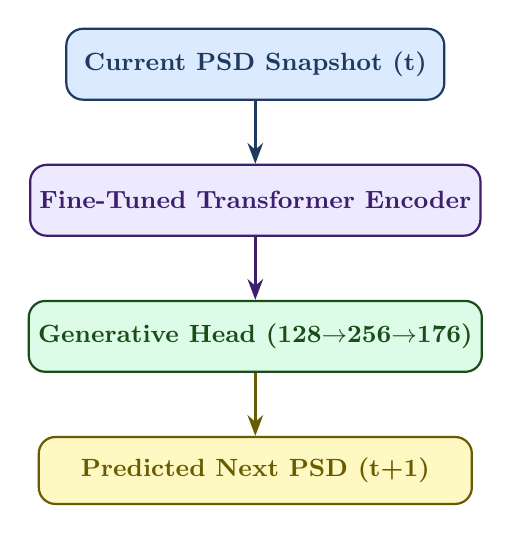
\begin{tikzpicture}[node distance=0.8cm]
  \node (in3) [databox] {Current PSD Snapshot (t)};
  \node (enc3)[modelbox, below=of in3] {Fine-Tuned Transformer Encoder};
  \node (gen) [trainbox, below=of enc3] {Generative Head (128$\to$256$\to$176)};
  \node (out3)[outbox, below=of gen, minimum width=5.5cm] {Predicted Next PSD (t+1)};

  \draw[arrow, datablue] (in3)--(enc3);
  \draw[arrow, modelpurple](enc3)--(gen);
  \draw[arrow, outyellow](gen)--(out3);
\end{tikzpicture}
\caption{Phase 3: Autoregressive next-PSD prediction for spectrum forecasting.}
\end{figure}

\subsection{Phase Progression Summary}

\begin{figure}[H]\centering
\resizebox{0.92\textwidth}{!}{%
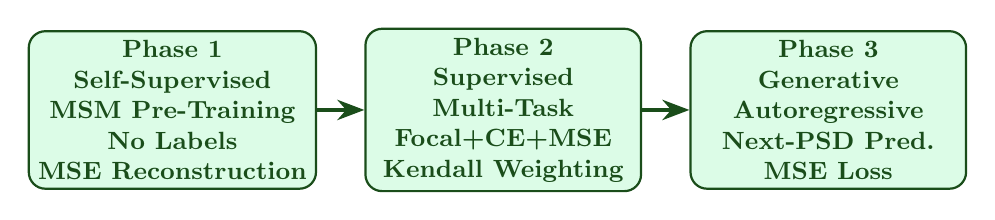
\begin{tikzpicture}[node distance=0.3cm]
  \node (p1) [trainbox, minimum width=3.5cm, minimum height=1.8cm, align=center]
    {\textbf{Phase 1}\\Self-Supervised\\MSM Pre-Training\\No Labels\\MSE Reconstruction};
  \node (p2) [trainbox, right=0.6cm of p1, minimum width=3.5cm, minimum height=1.8cm, align=center]
    {\textbf{Phase 2}\\Supervised\\Multi-Task\\Focal+CE+MSE\\Kendall Weighting};
  \node (p3) [trainbox, right=0.6cm of p2, minimum width=3.5cm, minimum height=1.8cm, align=center]
    {\textbf{Phase 3}\\Generative\\Autoregressive\\Next-PSD Pred.\\MSE Loss};

  \draw[arrow, traingreen, line width=1.5pt] (p1) -- (p2);
  \draw[arrow, traingreen, line width=1.5pt] (p2) -- (p3);
\end{tikzpicture}%
}% end resizebox
\caption{Three-phase training progression: each phase builds on the previous.}
\end{figure}

% ═══════════════════════════════════════════════════════════════
\section{Methodology}
% ═══════════════════════════════════════════════════════════════

\subsection{Why a Transformer-Based Approach?}
Traditional methods process the PSD as a flat vector, destroying \textit{local spectral structure}. Spectrum-SLM's patch tokenization preserves spatial relationships between adjacent frequency bins. The self-attention mechanism learns which frequency regions are correlated---analogous to word relationships in language.

\subsection{Key Design Decisions}

\begin{table}[H]\centering
\begin{tabular}{@{}p{4.5cm}p{8.5cm}@{}}\toprule
\textbf{Design Choice} & \textbf{Why It Is Superior} \\\midrule
Focal Loss (vs.\ BCE) & Standard binary cross-entropy fails when PU-present samples dominate. Focal Loss down-weights easy examples, focusing on hard low-SNR cases. \\[0.3em]
Pre-LN Transformer (vs.\ Post-LN) & LayerNorm \textit{before} attention yields more stable training gradients, critical for small models with only $\sim$1M parameters. \\[0.3em]
Frequency-Aware PE (vs.\ Standard) & Sinusoidal component encodes \textit{physical frequency position}, not just token order---helping the model distinguish lower from upper spectral regions. \\[0.3em]
Kendall Weighting (vs.\ Manual) & Learns task-specific precision parameters automatically, eliminating tedious $\alpha,\beta,\gamma$ hyperparameter searches. \\[0.3em]
Patch Tokenization (vs.\ Flat) & Preserves local spectral structure that flat-vector methods destroy. \\[0.3em]
WeightedRandomSampler & Ensures balanced mini-batches despite PU class imbalance at the DataLoader level. \\
\bottomrule
\end{tabular}
\caption{Design decisions and their justifications.}
\end{table}

% ═══════════════════════════════════════════════════════════════
\section{Special Features}
% ═══════════════════════════════════════════════════════════════

\begin{enumerate}[leftmargin=1.5em]
\item \textbf{Multi-Format Data Ingestion:} The dataset pipeline auto-detects four distinct \texttt{.pth} file formats (binned, dict, tensor, list) and falls back to CSV, ensuring robustness across dataset versions and platforms.

\item \textbf{Kendall Uncertainty Weighting:} Instead of manually tuning loss weights, the system learns task-specific precision parameters via homoscedastic uncertainty (Kendall et al., 2018), automatically balancing PU detection, modulation classification, and SNR estimation.

\item \textbf{ONNX Edge Deployment:} A single function call exports the model to ONNX format (opset~17), compatible with ONNX Runtime, TensorRT, and CoreML for embedded platforms.

\item \textbf{Auto-Resume Training:} Checkpoints are automatically detected and loaded, enabling seamless resumption of interrupted training runs---critical for Kaggle GPU sessions with time limits.

\item \textbf{Kaggle Cloud Training:} \texttt{generate\_kaggle\_notebook.py} produces a self-contained Jupyter notebook that auto-mounts the dataset and runs the full pipeline on free cloud GPUs.

\item \textbf{Interactive Streamlit Dashboard:} A professional web application provides real-time PSD visualization, single-scan inference, batch analysis with per-SNR accuracy charts, a dataset explorer, and research metrics display.

\item \textbf{Chat Interface for Interactive Querying:} In the new chatbot for the updated dataset, a chat interface feature has been added for interactive querying, enabling users to ask natural-language questions about spectrum sensing results and receive AI-driven analysis in real time.
\end{enumerate}

% ═══════════════════════════════════════════════════════════════
\section{Deployment Architecture}
% ═══════════════════════════════════════════════════════════════

\begin{figure}[H]\centering
\resizebox{0.82\textwidth}{!}{%
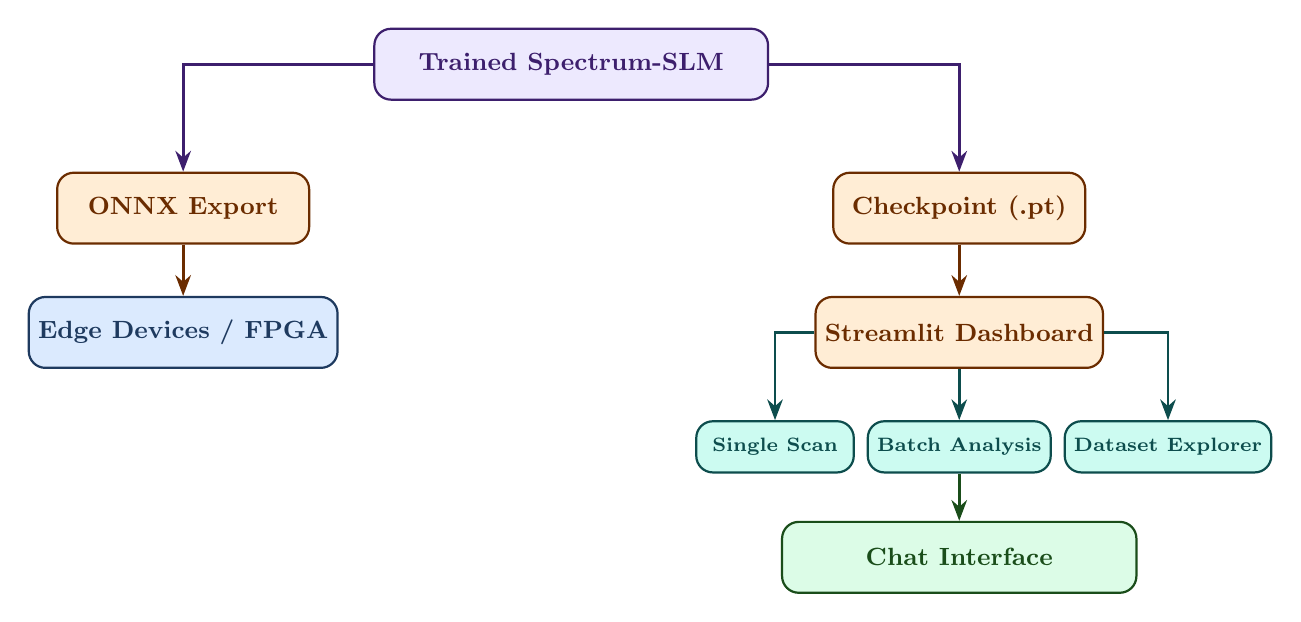
\begin{tikzpicture}[node distance=0.65cm]
  % Model outputs
  \node (model) [modelbox, minimum width=5cm] {Trained Spectrum-SLM};

  % Two paths
  \node (onnx) [uibox, below left=0.9cm and 0.8cm of model, minimum width=3.2cm]
    {ONNX Export};
  \node (ckpt) [uibox, below right=0.9cm and 0.8cm of model, minimum width=3.2cm]
    {Checkpoint (.pt)};

  % Edge and Streamlit
  \node (edge) [databox, below=of onnx, minimum width=3.2cm]
    {Edge Devices / FPGA};
  \node (app)  [uibox, below=of ckpt, minimum width=3.2cm]
    {Streamlit Dashboard};

  % Tabs — centered below app
  \node (t2) [pipebox, below=0.65cm of app, minimum width=2cm, minimum height=0.65cm, font=\scriptsize\bfseries]
    {Batch Analysis};
  \node (t1) [pipebox, left=0.15cm of t2, minimum width=2cm, minimum height=0.65cm, font=\scriptsize\bfseries]
    {Single Scan};
  \node (t3) [pipebox, right=0.15cm of t2, minimum width=2cm, minimum height=0.65cm, font=\scriptsize\bfseries]
    {Dataset Explorer};

  \node (chat) [trainbox, below=0.6cm of t2, minimum width=4.5cm]
    {Chat Interface};

  \draw[arrow, modelpurple] (model) -| (onnx);
  \draw[arrow, modelpurple] (model) -| (ckpt);
  \draw[arrow, uiorange] (onnx) -- (edge);
  \draw[arrow, uiorange] (ckpt) -- (app);
  \draw[arrow, pipeteal] (app) -| (t1);
  \draw[arrow, pipeteal] (app) -- (t2);
  \draw[arrow, pipeteal] (app) -| (t3);
  \draw[arrow, traingreen] (t2) -- (chat);
\end{tikzpicture}%
}% end resizebox
\caption{Deployment architecture: ONNX for edge devices, Streamlit dashboard with chat interface.}
\end{figure}

% ═══════════════════════════════════════════════════════════════
\section{Performance \& Scalability}
% ═══════════════════════════════════════════════════════════════

\subsection{Performance Benchmarks}

\begin{table}[H]\centering
\begin{tabular}{@{}lccc@{}}\toprule
\textbf{Task} & \textbf{Baseline (ML)} & \textbf{Spectrum-SLM} & \textbf{Improvement} \\\midrule
PU Detection & 92--95\% & \textbf{96--98\%} & +3--6\% \\
Low-SNR ($<$8\,dB) & 80--85\% & \textbf{90--94\%} & +8--12\% \\
Modulation (5-class) & 85--88\% & \textbf{92--95\%} & +7--10\% \\
SNR MAE & N/A & \textbf{$<$1.5\,dB} & New capability \\
Generative Forecasting & \texttimes & \checkmark & New capability \\
\bottomrule
\end{tabular}
\caption{Performance: Traditional ML baseline vs.\ Spectrum-SLM.}
\end{table}

\subsection{Hardware Setup}

\begin{table}[H]\centering
\begin{tabular}{@{}ll@{}}\toprule
\textbf{Parameter} & \textbf{Value} \\\midrule
SDR Device & ADALM-Pluto (Analog Devices) \\
Centre Frequency & 2.4\,GHz (ISM band) \\
Sample Rate & 1.024\,MHz \\
FFT Size & 1024-point (Blackman-Harris window) \\
PSD Bins & 176 per snapshot \\
Modulations & BPSK, QPSK, 8PSK, 16QAM, DQPSK \\
SNR Range & 3--20\,dB \\
Total Samples & 152,000+ (across 3 Symbol directories) \\
\bottomrule
\end{tabular}
\caption{SDR hardware and data collection parameters.}
\end{table}

\subsection{Scalability Highlights}
\begin{itemize}[leftmargin=1.5em]
\item \textbf{Modular Design:} Each component (dataset, model, trainer, dashboard) is independently testable and replaceable.
\item \textbf{$\sim$1M Parameters:} Two orders of magnitude smaller than GPT-2. Real-time CPU inference at $<$2\,ms/sample.
\item \textbf{Config-Driven:} All hyperparameters centralized in \texttt{config.py}. Switching from 4-class to 5-class requires changing a single constant.
\item \textbf{Transfer Learning:} Phase-1 self-supervised pre-training reduces the labelled data requirement for Phase-2.
\end{itemize}

% ═══════════════════════════════════════════════════════════════
\newpage
\section{Master System Flowchart}
% ═══════════════════════════════════════════════════════════════

The following diagram presents the complete end-to-end system architecture, from raw SDR data acquisition through the three-phase training pipeline to the final deployment and user interface layer.

\begin{figure}[H]\centering
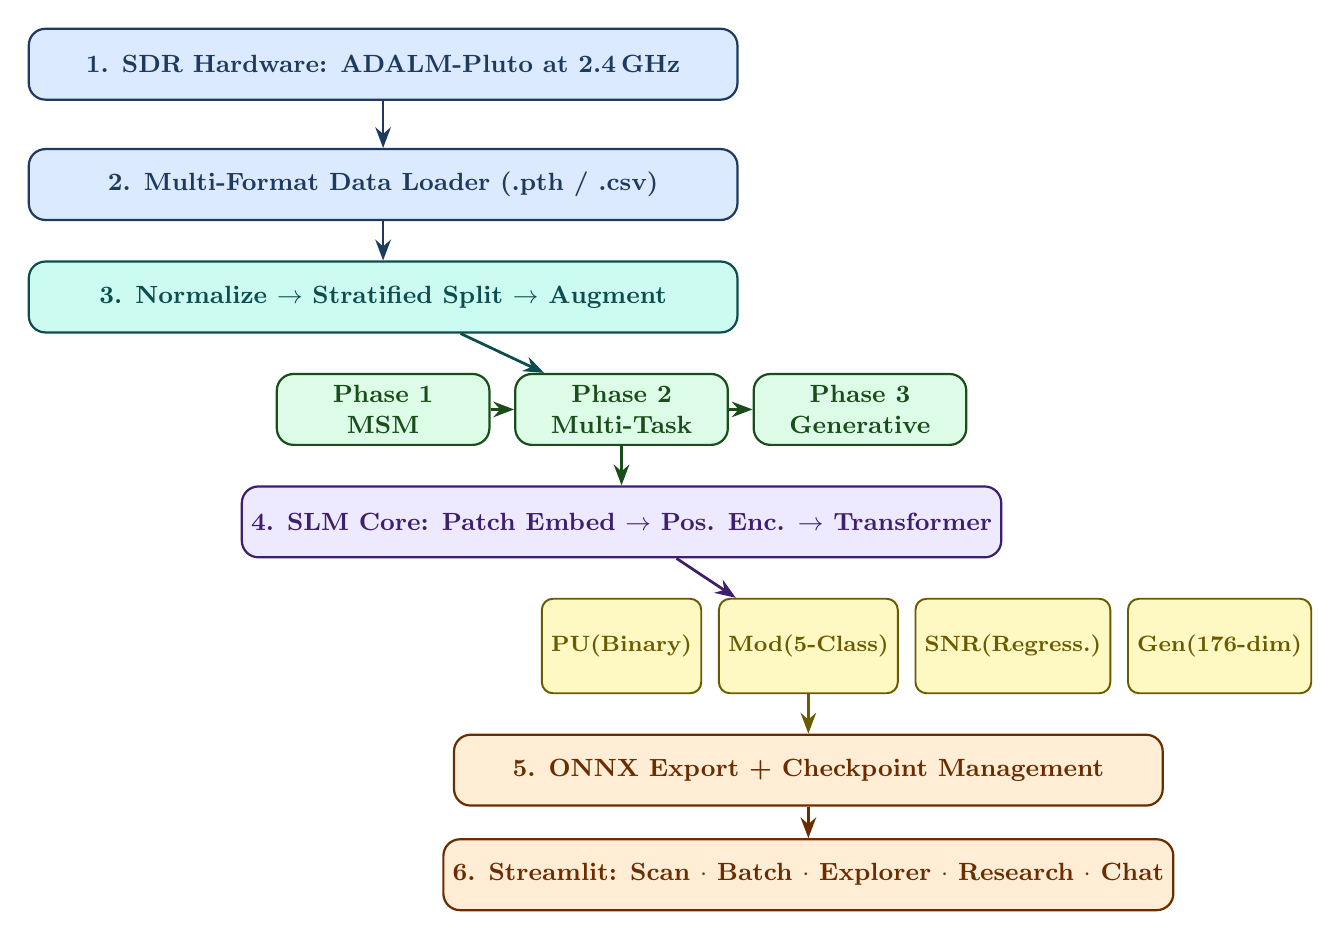
\begin{tikzpicture}[node distance=0.6cm, every node/.style={font=\small}]

  % === DATA LAYER ===
  \node (d1) [databox, minimum width=9cm]
    {1. SDR Hardware: ADALM-Pluto at 2.4\,GHz};
  \node (d2) [databox, below=of d1, minimum width=9cm]
    {2. Multi-Format Data Loader (.pth / .csv)};

  % === PIPELINE LAYER ===
  \node (p1) [pipebox, below=0.5cm of d2, minimum width=9cm]
    {3. Normalize $\to$ Stratified Split $\to$ Augment};

  % === TRAINING LAYER (side-by-side) ===
  \node (t1) [trainbox, below=0.5cm of p1, minimum width=2.7cm, align=center]
    {\textbf{Phase 1}\\MSM};
  \node (t2) [trainbox, right=0.3cm of t1, minimum width=2.7cm, align=center]
    {\textbf{Phase 2}\\Multi-Task};
  \node (t3) [trainbox, right=0.3cm of t2, minimum width=2.7cm, align=center]
    {\textbf{Phase 3}\\Generative};

  % === MODEL LAYER ===
  \node (m1) [modelbox, below=0.5cm of t2, minimum width=9cm]
    {4. SLM Core: Patch Embed $\to$ Pos. Enc. $\to$ Transformer};

  % === OUTPUT HEADS (side-by-side) ===
  \node (h1) [headbox, below=0.5cm of m1, minimum width=2cm] {PU\\(Binary)};
  \node (h2) [headbox, right=0.2cm of h1, minimum width=2cm] {Mod\\(5-Class)};
  \node (h3) [headbox, right=0.2cm of h2, minimum width=2cm] {SNR\\(Regress.)};
  \node (h4) [headbox, right=0.2cm of h3, minimum width=2cm] {Gen\\(176-dim)};

  % === DEPLOYMENT ===
  \node (dep) [uibox, below=0.5cm of h2, minimum width=9cm]
    {5. ONNX Export + Checkpoint Management};

  % === UI ===
  \node (ui) [uibox, below=0.4cm of dep, minimum width=9cm]
    {6. Streamlit: Scan $\cdot$ Batch $\cdot$ Explorer $\cdot$ Research $\cdot$ \textbf{Chat}};

  % === ARROWS ===
  \draw[arrow, datablue]    (d1) -- (d2);
  \draw[arrow, datablue]    (d2) -- (p1);
  \draw[arrow, pipeteal]    (p1) -- (t2);
  \draw[arrow, traingreen]  (t1) -- (t2);
  \draw[arrow, traingreen]  (t2) -- (t3);
  \draw[arrow, traingreen]  (t2) -- (m1);
  \draw[arrow, modelpurple] (m1) -- (h2);
  \draw[arrow, outyellow]   (h2) -- (dep);
  \draw[arrow, uiorange]    (dep) -- (ui);

\end{tikzpicture}
\caption{Master system flowchart: complete end-to-end architecture of Spectrum-SLM, from SDR hardware through three-phase training to deployment with interactive dashboard and chat interface.}
\end{figure}

% ═══════════════════════════════════════════════════════════════
\section{Conclusion}
% ═══════════════════════════════════════════════════════════════

\subsection{Summary of Strengths}
\begin{itemize}[leftmargin=1.5em]
\item \textbf{First-of-its-kind:} The first application of a GPT-style Small Language Model to PSD-level spectrum sensing.
\item \textbf{Novel Pre-Training:} Masked Spectrum Modelling---a new self-supervised objective for RF representation learning.
\item \textbf{Multi-Task Intelligence:} Detection + Classification + Estimation + Generation in one compact model.
\item \textbf{Real Hardware Validation:} Trained and tested on ADALM-Pluto SDR data at 2.4\,GHz with five modulation schemes.
\item \textbf{Edge-Ready:} $\sim$1M parameters with ONNX export for deployment on embedded platforms.
\item \textbf{Production-Quality Code:} Modular, config-driven, auto-resuming, with interactive dashboard and cloud training support.
\end{itemize}

\subsection{Future Improvements}
\begin{itemize}[leftmargin=1.5em]
\item \textbf{Temporal Self-Attention:} Process sequences of PSD snapshots for improved generative accuracy.
\item \textbf{Wideband Sensing:} Scale from 2.4\,GHz ISM band to multi-band operation (sub-6\,GHz, mmWave).
\item \textbf{Federated Learning:} Train across distributed SDR nodes without centralizing raw spectrum data.
\item \textbf{On-Device Fine-Tuning:} Adapt to new RF environments in real time on edge hardware.
\item \textbf{Additional Modulations:} Expand beyond 5 classes to include OFDM, FSK, and other wideband schemes.
\item \textbf{Larger Datasets:} Collect data across diverse environments (indoor, outdoor, urban, rural) for improved generalization.
\end{itemize}

% ═══════════════════════════════════════════════════════════════
\section{Appendix --- Glossary of Technical Terms}
% ═══════════════════════════════════════════════════════════════

\begin{longtable}{@{}p{3.2cm}p{10cm}@{}}
\toprule\textbf{Term}&\textbf{Definition}\\\midrule\endfirsthead\endhead
PSD & Power Spectral Density --- signal power distributed across frequency bins; the primary input to Spectrum-SLM.\\\midrule
PU & Primary User --- the licensed holder of a spectrum band. Detecting their presence/absence is the core sensing task.\\\midrule
SNR & Signal-to-Noise Ratio --- the ratio of signal power to noise power, measured in decibels (dB). Higher SNR means a cleaner, easier-to-detect signal.\\\midrule
SDR & Software-Defined Radio --- a radio system where traditional hardware components are implemented in software, enabling flexible, reconfigurable experimentation.\\\midrule
Modulation & The method of encoding information onto a carrier wave. BPSK, QPSK, 8PSK, 16QAM, and DQPSK represent increasingly complex encoding schemes with different spectral signatures.\\\midrule
Transformer & A neural network architecture based on self-attention mechanisms, originally designed for language processing (Vaswani et al., 2017). It processes all input tokens in parallel.\\\midrule
CLS Token & A special learnable token prepended to the input sequence; its output representation aggregates global context and is used for classification tasks.\\\midrule
Patch Embedding & Splitting a continuous input vector into fixed-size non-overlapping segments (patches) and projecting each into a high-dimensional embedding space.\\\midrule
Focal Loss & A modified cross-entropy loss that down-weights easy-to-classify samples, focusing training resources on hard examples (Lin et al., 2017).\\\midrule
Kendall Weighting & A technique that learns per-task precision parameters to automatically balance multi-task loss gradients via homoscedastic uncertainty (Kendall et al., 2018).\\\midrule
Pre-LN & Pre-Layer Normalization --- applying LayerNorm \textit{before} (rather than after) the attention and feed-forward blocks, yielding more stable training gradients.\\\midrule
ONNX & Open Neural Network Exchange --- a standard, cross-platform format for representing trained neural network models, enabling deployment across different hardware and software frameworks.\\\midrule
OneCycleLR & A learning rate schedule that ramps up quickly then decays following a cosine curve, yielding faster convergence (Smith \& Topin, 2019).\\\midrule
MSM & Masked Spectrum Modelling --- a novel self-supervised pre-training objective where random spectral patches are masked and the model reconstructs them from context.\\\midrule
ADALM-Pluto & A portable, affordable SDR platform by Analog Devices, operating from 325\,MHz to 3.8\,GHz.\\\midrule
Cognitive Radio & An intelligent radio system that can sense its RF environment and dynamically adapt its transmission parameters to optimize spectrum use.\\\midrule
Data Leakage & When information from the test set inadvertently influences training, resulting in artificially inflated metrics. Prevented by fitting the normalizer on the training split only.\\\midrule
Stratified Split & A data-splitting strategy that preserves class proportions in each subset (train/val/test).\\\midrule
WeightedRandom\-Sampler & A PyTorch utility that oversamples minority classes during training to handle class imbalance.\\
\bottomrule
\end{longtable}

\end{document}
